\Problem{Interpreting a Potential Energy Graph}{\InterPotEG}{
A particle with the potential energy shown in the graph is moving to the right at $ x = 0 $ m with total energy $ E $.
}
\ProblemFig{\InterPotEGFig}{
\centering
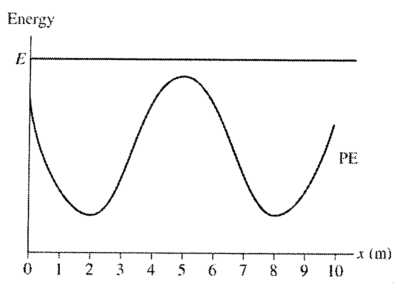
\includegraphics{\FileDepth/Activities/Interpreting_a_Potential_Energy_Graph/PE_Graph_to_Interpret.pdf}
}
\ProblemSub{\InterPotEGA}{
(a) At what value or values of $ x $ is the particle's speed a maximum?
}
\Solution{\InterPotEGASol}{

At 2 m and 8 m, where the potential energy is smallest.
}
\ProblemSub{\InterPotEGB}{
(b) At what value or values of $ x $ is the particle's speed a minimum?
}
\Solution{\InterPotEGBSol}{

At 5 m, where the potential energy is largest.
}
\ProblemSub{\InterPotEGC}{
(c) At what value or values of $ x $ is the potential energy a maximum?
}
\Solution{\InterPotEGCSol}{

At 5 m.
}
\ProblemSub{\InterPotEGD}{
(d) Does this particle have a turning point in the range of $ x $ covered by the graph? If so, where?
}
\Solution{\InterPotEGDSol}{

There are no turning points, as the potential energy never crosses the total energy line.
}
\ProblemSub{\InterPotEGE}{
(e) In which intervals of $ x $ is the force on the particle to the right?
}
\Solution{\InterPotEGESol}{

Since $ F_{x} = -\frac{dU}{dx} $ (negative of slope), we know that the force is to the right ($ F_{x} $ is positive) from 0 m to 2 m and from 5 m to 8 m.
}
\ProblemSub{\InterPotEGF}{
(f) In which intervals of $ x $ is the force on the particle to the left?
}
\Solution{\InterPotEGFSol}{

The force is to the left ($ F_{x} $ is negative) from 2 m to 5 m and from 8 m to 10 m.
}
\ProblemSub{\InterPotEGG}{
(g) At what value or values of $ x $ is the magnitude of the force a maximum?
}
\Solution{\InterPotEGGSol}{

When the slope of $ U $ versus $ x $ is steepest: $ x = 0 $ m, 3.5 m, 6.5 m, and 10 m.
}
\ProblemSub{\InterPotEGH}{
(h) At what value or values of $ x $ are positions of stable equilibrium?
}
\Solution{\InterPotEGHSol}{

Equilibrium occurs when $ F_{x} = 0 $ N. Stable equilibrium occurs when the force felt on either side of the point pushes the particle back toward the point. This happens at the minima of potential energy: $ x = 2 $ m and 8 m.
}
\ProblemSub{\InterPotEGI}{
(i) At what value or values of $ x $ are positions of unstable equilibrium?
}
\Solution{\InterPotEGISol}{

Unstable equilibrium occurs when the force felt on either side of the equilibrium point pushes the particle away from the point. This happens at the maximum of potential energy: $ x = 5 $ m.
}
\ProblemSub{\InterPotEGJ}{
(j) If the particle is released from rest at $ x = 0 $ m, will it reach $ x = 10 m $? Explain.
}
\Solution{\InterPotEGJSol}{

No. If released from rest, the particle's total energy is the initial potential energy and can never exceed this value. The particle will turn around at about $ x = 3.5 $ m.
}